\documentclass[a4paper,fleqn]{cas-dc}

\usepackage[authoryear,longnamesfirst]{natbib}

\hbadness=1000
\vbadness=1000
\raggedbottom
\sloppy

\begin{document}

\let\WriteBookmarks\relax
\def\floatpagepagefraction{1}
\def\textpagefraction{.001}

\shorttitle{Delay Propagation in Indian Railways}
\shortauthors{A. Sarje et al.}

\title[mode=title]{Data-Centric Approach to Train Delay Prediction in Indian Railways}

\author[1]{Arjun Sarje}[orcid=0009-0000-0563-1977]
\cormark[1]
\ead{arjun.sarje8055@gmail.com}

\author[1]{Ashvin Sukaye}
\ead{ashvinsukaye@gmail.com}

\author[1]{Rashi Kumar}[orcid=0000-0002-4497-6481]
\ead{rashi.ai@satiengg.in}

\affiliation[1]{organization={Department of Artificial Intelligence,
                           Samrat Ashok Technological Institute},
                addressline={Vidisha},
                postcode={470229},
                state={Madhya Pradesh},
                country={India}}

\cortext[1]{Corresponding author}

\begin{abstract}
Delay analytics for Indian Railways is constrained by the absence of a
reproducible, station-level, machine-learning-ready dataset. This paper
addresses that gap with a data-centric pipeline that was designed, deployed,
and operated before any predictive modelling was attempted. Scheduled
workflows poll a live train-tracking application programming interface and
persist station-level scheduled and actual timestamps, together with arrival
and departure delays, into a cloud relational database using an idempotent,
fault-aware design with explicit journey lifecycle tracking. Between January
and June 2026 the pipeline ran continuously for a fixed panel of ten trains
covering single-day and multi-day services, yielding more than 61{,}000
unique station-level records. Exploratory analysis shows that delay behaviour
is strongly segment-dependent: some adjacent halt pairs persistently add delay
while others persistently absorb it, suggesting candidate operational differences
such as congested locations versus segments with recovery margin. This is quantified
by a station-pair delay-delta indicator, $\alpha$, which classifies route
segments into delay-adding, neutral, and recovery zones and is reported
together with an observation-coverage ratio. Baseline next-station delay
prediction on held-out journeys reaches a mean absolute error of 4.78\,min
with a temporal convolutional network, 43\,\% below a naive persistence
baseline, while simpler statistical and tree baselines fail to improve on
persistence. Percentage-based error is shown to be unusable for this target
because of near-zero delay denominators. The outcome of this phase is a
documented dataset-generation infrastructure, an interpretable segment-level
diagnostic for where delay arises operationally, and benchmarked forecasts 
addressed in subsequent work.
\end{abstract}

\begin{highlights}
\item Automated pipeline collected over 61,000 station-level delay records
\item Station-pair alpha separates delay-adding from delay-recovery segments
\item Best next-station model: MAE 4.78 min, RMSE 8.1 min on held-out journeys
\item Reproducible open data-generation pipeline for Indian Railways
\end{highlights}

\begin{keywords}
delay propagation \sep Indian Railways \sep data-centric pipeline \sep
station-level delay data \sep sequence models \sep timetable reliability
\end{keywords}

\maketitle

\section{Introduction}

\subsection{Background and need}
Indian Railways operates one of the largest rail networks in the world,
carrying more than 8 billion passenger journeys annually over approximately
68{,}000~km of route \citep{indian_railways_stats}, and is correspondingly
sensitive to delay propagation across stations and routes. A delay introduced
on one segment is frequently carried forward, amplified, or partially absorbed
as the service proceeds, affecting rolling-stock reuse, crew and platform
scheduling, and downstream connectivity. Two services sharing the same
corridor may therefore end with very different delay profiles, depending on
the segments traversed and where recovery capacity exists along the route.

Despite this operational scale, no openly accessible, continuously updated,
and methodologically reproducible station-level dataset exists for delay
analytics. Existing studies are often constrained to coarse aggregated
reports, manual surveys prone to sampling bias, or inaccessible proprietary
sources. This matters directly for modeling, because delay-prediction quality
depends heavily on consistent, long-duration data that preserves journey
context. A model trained on a short snapshot, or on inconsistently ordered
station records, cannot reliably separate persistent route-level effects from
one-off operational disturbances.

This project therefore began with a data-centric goal: build a reliable
automated collection pipeline first, and only then use the collected dataset
for exploratory analytics and predictive modeling. The goal covers both
operational diagnosis (where delay accumulates and where it is recovered) and
forecasting (how much delay carries forward to the next station). Framing the
problem this way also makes the resulting dataset reusable for research
questions beyond the immediate forecasting objective, such as route-level
diagnosis and segment benchmarking.

\subsection{Project motivation}
Unlike European and Japanese systems with open operational feeds, the Indian
context lacks station-level, lifecycle-complete delay traces. This motivated
a reproducible collection pipeline with documented methodology to answer two
complementary questions. First, an operational question: why trains get late
at specific locations, for example where station congestion, platform
occupancy, or limited running-time margin causes delay to accumulate, and
where timetable slack allows it to be recovered. Second, a predictive
question: how much of the observed delay will carry forward to the next
station. The station-pair analysis in this paper addresses the first question
by locating persistent delay-adding and recovery zones, treated as candidate
operational effects to be confirmed with concurrent multi-train station data
rather than proven root causes (future work), while the baseline models
address the second question by benchmarking
next-station forecasts. The first phase of this work was presented at
Technovision 2026 at Samrat Ashok Technological Institute (SATI), Vidisha,
and received the first prize in the Artificial Intelligence and Data Science
(AI\&DS) domain.

\subsection{Objectives}
The key objectives of this work are:
\begin{enumerate}
    \item to build a scalable, automated, and reproducible pipeline that
          collects station-level delay data for selected trains;
    \item to maintain journey lifecycle tracking so that completion and
          failure context is preserved;
    \item to perform train-wise exploratory analysis that locates where
          delay systematically grows or shrinks along a route;
    \item to quantify station-segment behavior using a robust route-level
          metric ($\alpha$) as an operational diagnostic for candidate
          delay-adding and recovery zones;
    \item to establish baseline delay-prediction models as a reference for
          future improvements;
    \item to document the collection methodology so that the dataset and
          results are reproducible and extensible.
\end{enumerate}

\subsection{Contributions in the current phase}
The main contributions of this phase are:
\begin{itemize}
    \item \textbf{Automated collection pipeline:} continuous operation
          since January 2026 with no manual intervention;
    \item \textbf{Station-level dataset:} more than 61{,}000 unique records
          collected from January to June 2026;
    \item \textbf{Exploratory data analysis workflow:} train-wise,
          halt-station-aligned delay-trend analysis for ten trains;
    \item \textbf{Station-pair alpha analysis:} identification of
          delay-add and delay-recovery zones along a route;
    \item \textbf{Modeling benchmarks:} random forest, polynomial
          regression, time-series trials (ARIMA, SARIMA, Prophet, Chronos),
          tuned gradient boosting (XGBoost), and sequence models (LSTM, TCN).
\end{itemize}

\subsection{Organization of the paper}
Section~\ref{sec:related} reviews related literature and identifies the
research gap. Section~\ref{sec:problem} formalizes the problem statement.
Section~\ref{sec:proposed} describes the proposed and implemented system
architecture and methodology. Section~\ref{sec:results} presents dataset
statistics, analysis results, alpha findings, baseline modeling outcomes,
and a comparison with prior work. Section~\ref{sec:conclusion} concludes the
current work and outlines future directions.

\section{Related work}
\label{sec:related}

\subsection{Railway delay modeling in the international context}
International railway systems such as those in the United Kingdom and
Germany provide open operational feeds that support reproducible analytics
\citep{uk_rail_data,german_rail_data}. Building on such feeds, prior studies
have applied machine learning and delay-propagation models for delay
forecasting and traffic optimization
\citep{oneto2018train,flier2009delay,goverde2010railway}. These datasets
typically include structured temporal events and multi-year coverage, which
makes replication and comparison of published results feasible and allows
models to be evaluated under controlled conditions. Rescheduling objectives with
passenger-dissatisfaction criteria have also been formulated, for example for
Japanese services \citep{tomii2005train}, although reported results are limited to
simulation studies rather than operationally collected traces.

\subsection{Indian context and data-availability gap}
For Indian Railways, meaningful research on delay prediction exists, but
reproducible open-data access remains limited. Gaurav and Srivastava proposed
a zero-shot Markov framework using data from 135 trains over March 2016 to
February 2018, yet the underlying dataset and source were not openly released
for direct reproduction \citep{gaurav2018zeroshot}. Arshad and Ahmed also
reported machine-learning-based delay prediction with data references to
online running-status sources, but without an openly shareable benchmark
dataset accompanying the publication \citep{arshad2019prediction}. More
recently, the RSTGCN study claimed a nationwide Indian railway delay dataset,
but at the time of review that dataset was not publicly accessible through
the links in the paper's repository trail, which limits independent
verification and reuse \citep{chowdhury2025rstgcn}. While high-level
operational reports do exist \citep{indian_railways_stats}, model-ready
station-level traces with continuous open access are still uncommon.

\subsection{Requirements implied by prior work}
Taken together, the studies above implicitly define the properties that a
usable delay dataset must satisfy. First, records must be station-level
rather than only train-level, because propagation is a segment-wise
phenomenon. Second, each record must carry journey context, so that
observations from different runs of the same service can be aligned and
compared. Third, the station ordering must be stable across journey dates,
otherwise segment-level comparisons are not meaningful. Fourth, the
observation horizon must be long enough to separate persistent effects from
transient ones. Finally, the collection process should be documented well
enough to be reproducible, since otherwise reported accuracy figures cannot
be independently validated.

\subsection{Comparative insight and research gap}
Most prior work emphasizes prediction models; however, prediction quality is
strongly data-dependent. In our case, delay forecasting was the intended
primary objective, but the lack of consistently accessible dataset
infrastructure became an enabling bottleneck that had to be solved first. The
literature therefore indicates that data quality, consistency, and
operational context are prerequisites for robust prediction. Accordingly,
this phase prioritizes systematic data generation and station-level
interpretability as a prerequisite stage, with forecasting-performance
improvement as the downstream target. In particular, this work contributes a
data-first collection and analysis pipeline for the Indian context and
introduces an interpretable station-pair alpha indicator for operational
insight prior to stronger model claims.

\section{Problem statement}
\label{sec:problem}

\subsection{Core problem}
The primary long-term problem is robust train delay forecasting for Indian
Railways, especially station-to-station delay propagation and
arrival-time reliability improvement. In practical execution, however, we
encountered an enabling problem first: the absence of sufficiently open,
continuously collected, station-level data needed to train and validate such
models.

\subsection{Observed challenges}
Several concrete challenges motivate this formulation:
\begin{itemize}
    \item open historical traces that preserve journey-state context are
          missing from available public sources;
    \item reproducible collection pipelines for Indian routes are rarely
          documented publicly;
    \item comparing station behavior across journey dates is difficult
          without a stable station ordering;
    \item baseline models struggle without route-aware feature design and
          normalized preprocessing;
    \item operational causes of lateness, such as congestion at specific
          stations or segments, cannot be fully attributed from single-train
          traces alone; concurrent multi-train station data are needed to
          confirm congestion effects;
    \item existing public-facing estimated-time-of-arrival systems are often
          perceived as heavily timetable- or heuristic-driven, which
          motivates a stronger data-driven alternative for delay-aware
          prediction.
\end{itemize}

Each of these challenges compounds the others. Without journey-state context,
abandoned or incomplete runs cannot be excluded, which biases any downstream
statistic. Without a stable station ordering, the same physical segment may
appear at different positions on different days, making segment-level
aggregation unreliable. And without normalized preprocessing, even a
well-specified model tends to fit dominant, high-delay segments at the expense
of the smaller recovery effects that are operationally informative.

\subsection{Formal problem statement}
The project problem is to design and operate an automated data pipeline that
collects reliable station-level delay data for selected Indian trains, and
then to develop a data analysis framework that can:
\begin{enumerate}
    \item reveal persistent station-segment delay behavior;
    \item quantify delay accumulation and delay-recovery zones; and
    \item provide benchmark delay-forecasting baselines for future model
          enhancement.
\end{enumerate}

\subsection{Relation to existing schemes}
Unlike approaches that begin directly with model training on limited
snapshots, this work first constructs a reproducible data foundation with
lifecycle tracking, idempotent storage, and explicit quality checks. This
directly addresses the enabling bottleneck---data availability---so that the
primary objective of better delay forecasting can subsequently be pursued
with stronger evidence. The same design also makes the collection process
auditable, because every stored record can be traced back to a specific
journey date and polling cycle.

\section{Proposed work: system architecture and methodology}
\label{sec:proposed}

\subsection{System overview}
The implemented system uses a serverless execution model driven by scheduled
workflows and cloud database storage. Two polling workflows are maintained:
one for single-day trains and one for multi-day trains, reflecting their
substantially different journey durations. Each workflow is triggered on a
fixed cron schedule through GitHub Actions---every 5~h for single-day trains
and every 12~h for multi-day trains---and executes a dedicated Python
polling script that queries the RailRadar API \citep{railradar_about} and
persists resulting records to a Supabase PostgreSQL database. Because
scheduling is external to the application code, collection continues without
manual intervention, and the same scripts can be redeployed locally for
verification or backfill. Keeping the two service classes on separate
schedules also ensures that long-distance services are not polled at a
cadence designed for short commuter runs.
Fig.~\ref{fig:arch} shows the overall collection architecture.

\begin{figure}[width=\columnwidth]
\centering
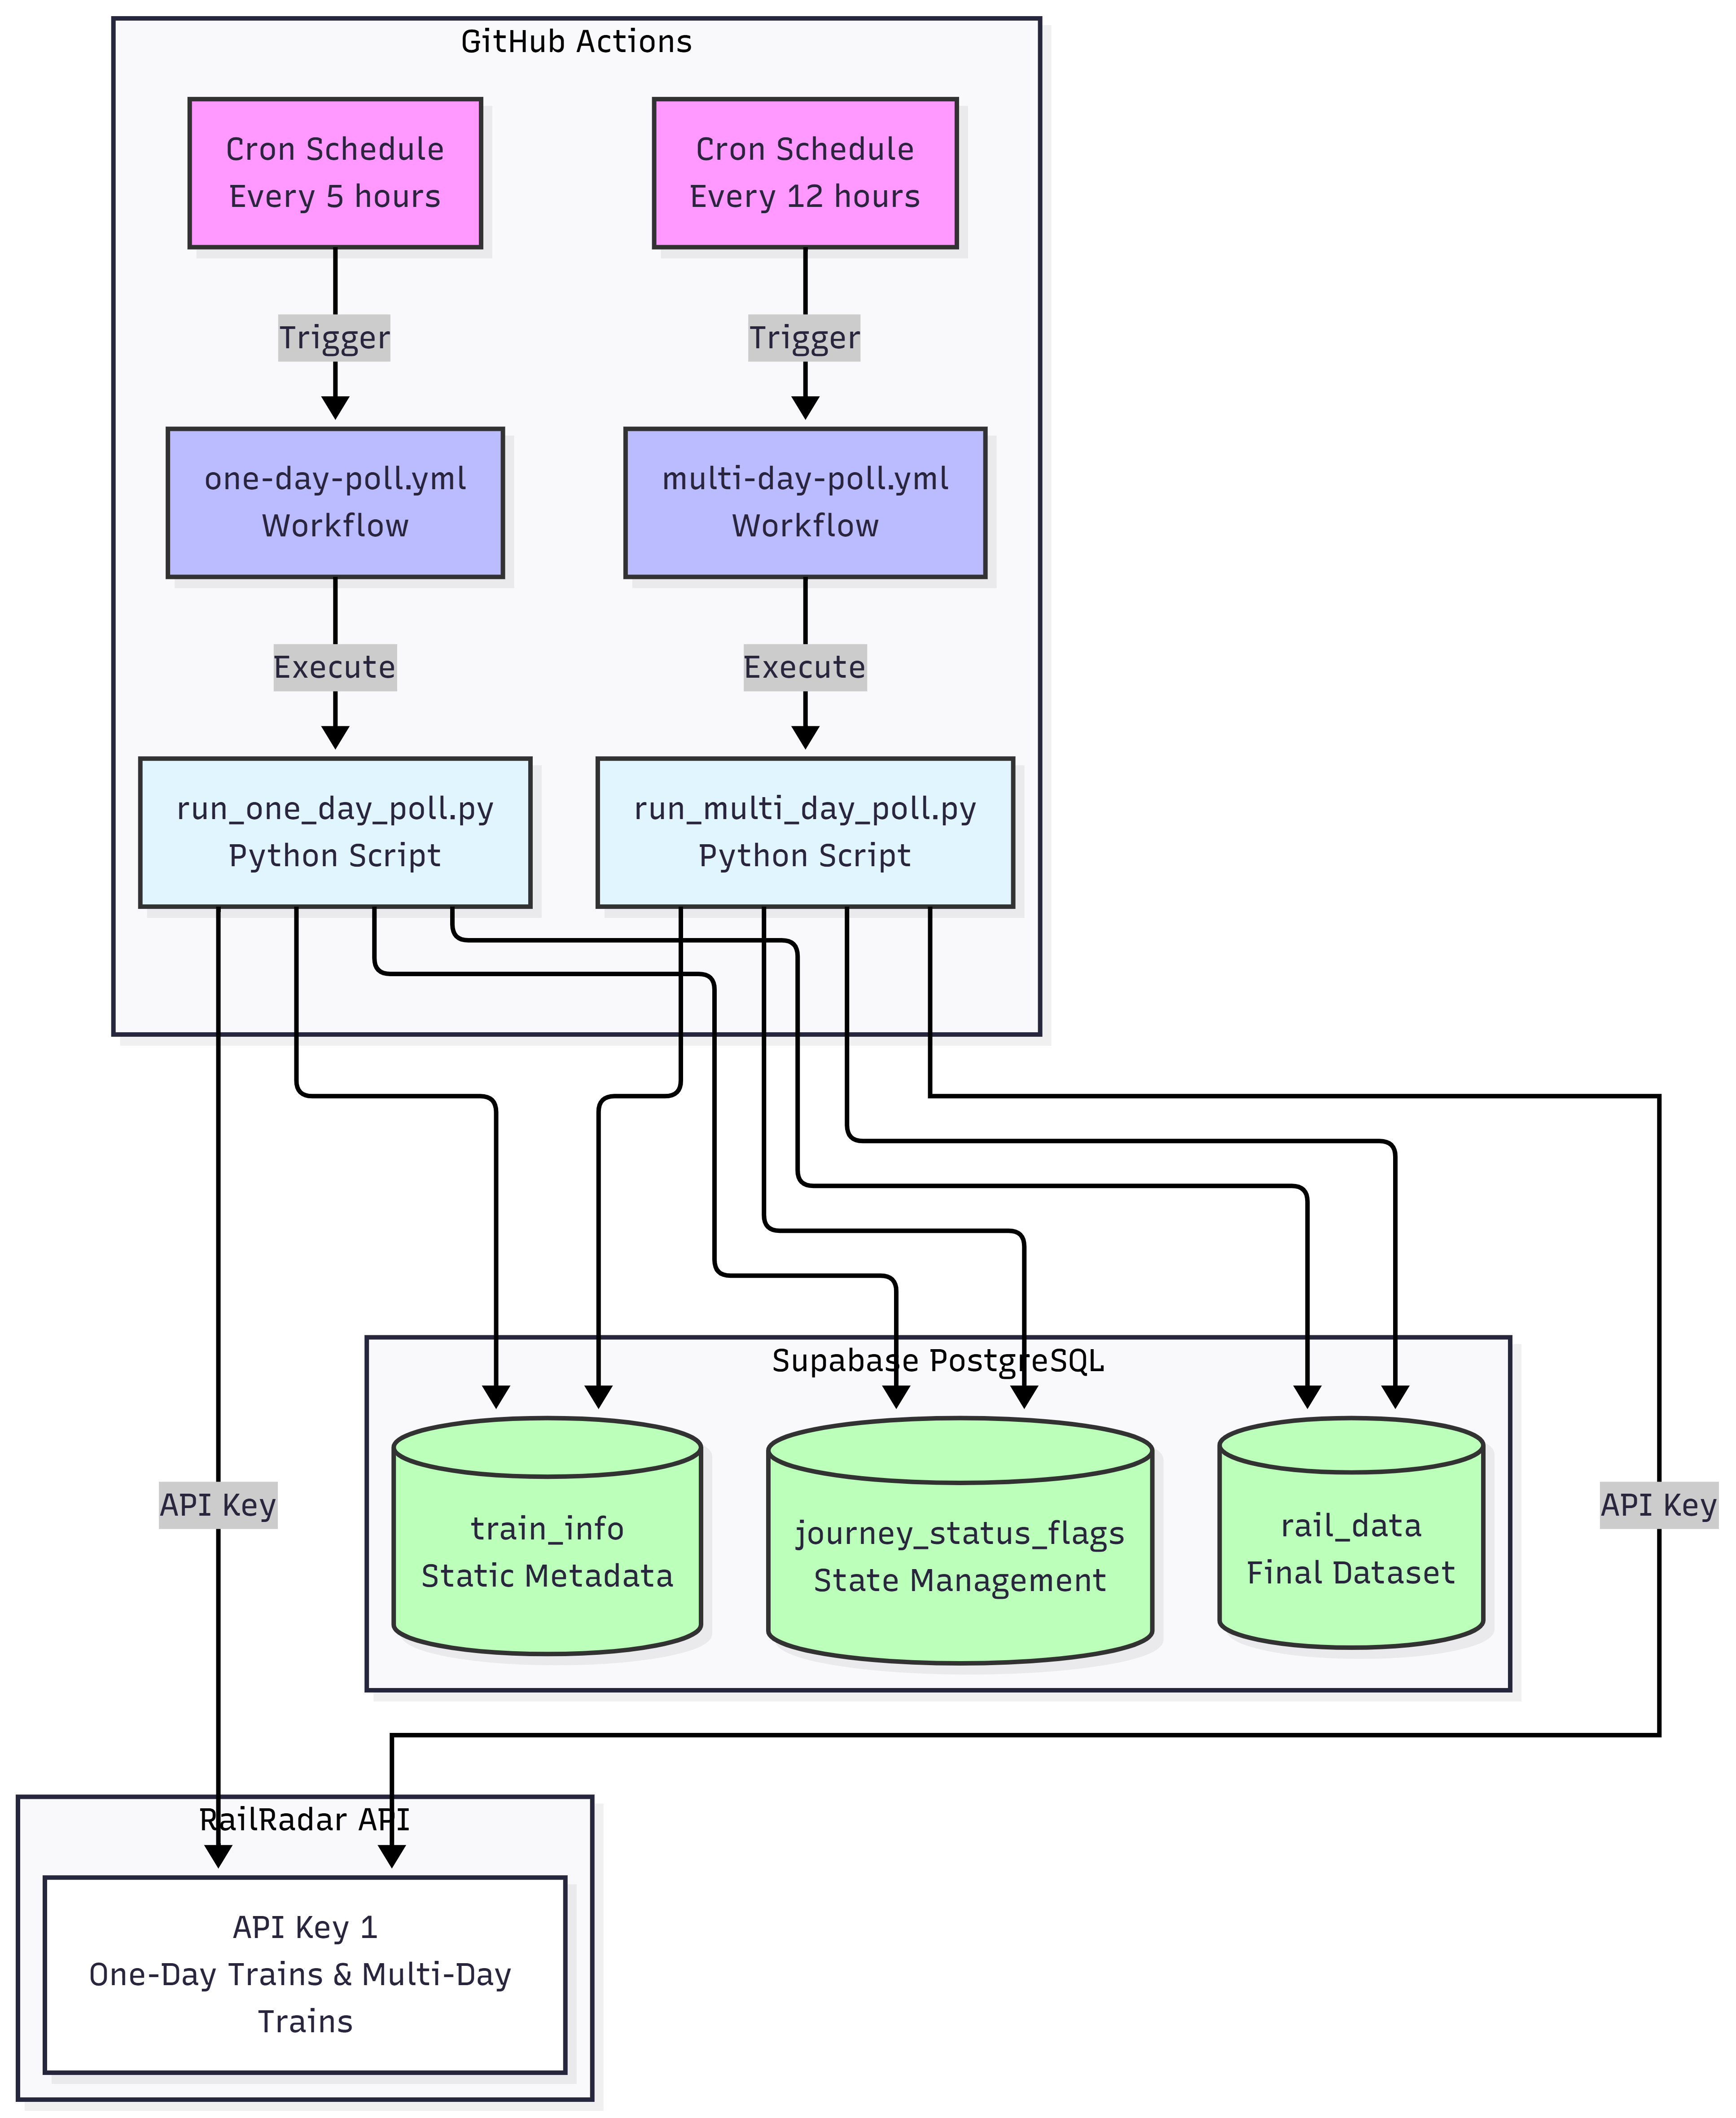
\includegraphics[width=\linewidth]{system_architecture.png}
\caption{Automated data-collection architecture integrating the scheduler, the
RailRadar API, and the database.}
\label{fig:arch}
\end{figure}

\subsection{Dual-phase polling methodology}
Collection proceeds in two phases.

\subsubsection{Phase 1: new-journey detection}
For each configured train, the pipeline checks whether a journey record
already exists for the current Indian Standard Time (IST) date. If not,
RailRadar live data is queried to confirm the journey's start conditions. On a
valid start, a new tracker row is inserted with initial flag values so that
the journey becomes eligible for ongoing polling.

\subsubsection{Phase 2: ongoing-journey tracking}
Every journey marked as neither completed nor abandoned is polled. Completion
is detected when the current station code matches the configured destination
code; on completion, the retrieved route station records are inserted into the
main dataset table. On repeated polling failures, the flag counter increases
and beyond a configured threshold eventually triggers abandonment of that
journey, without writing station-level data. This separation ensures that
incomplete or unreliable journeys never contaminate the analytical dataset,
while still preserving the fact that the journey occurred.
Fig.~\ref{fig:state_machine} shows the journey state machine used for this
lifecycle tracking.

\begin{figure}[width=\columnwidth]
\centering
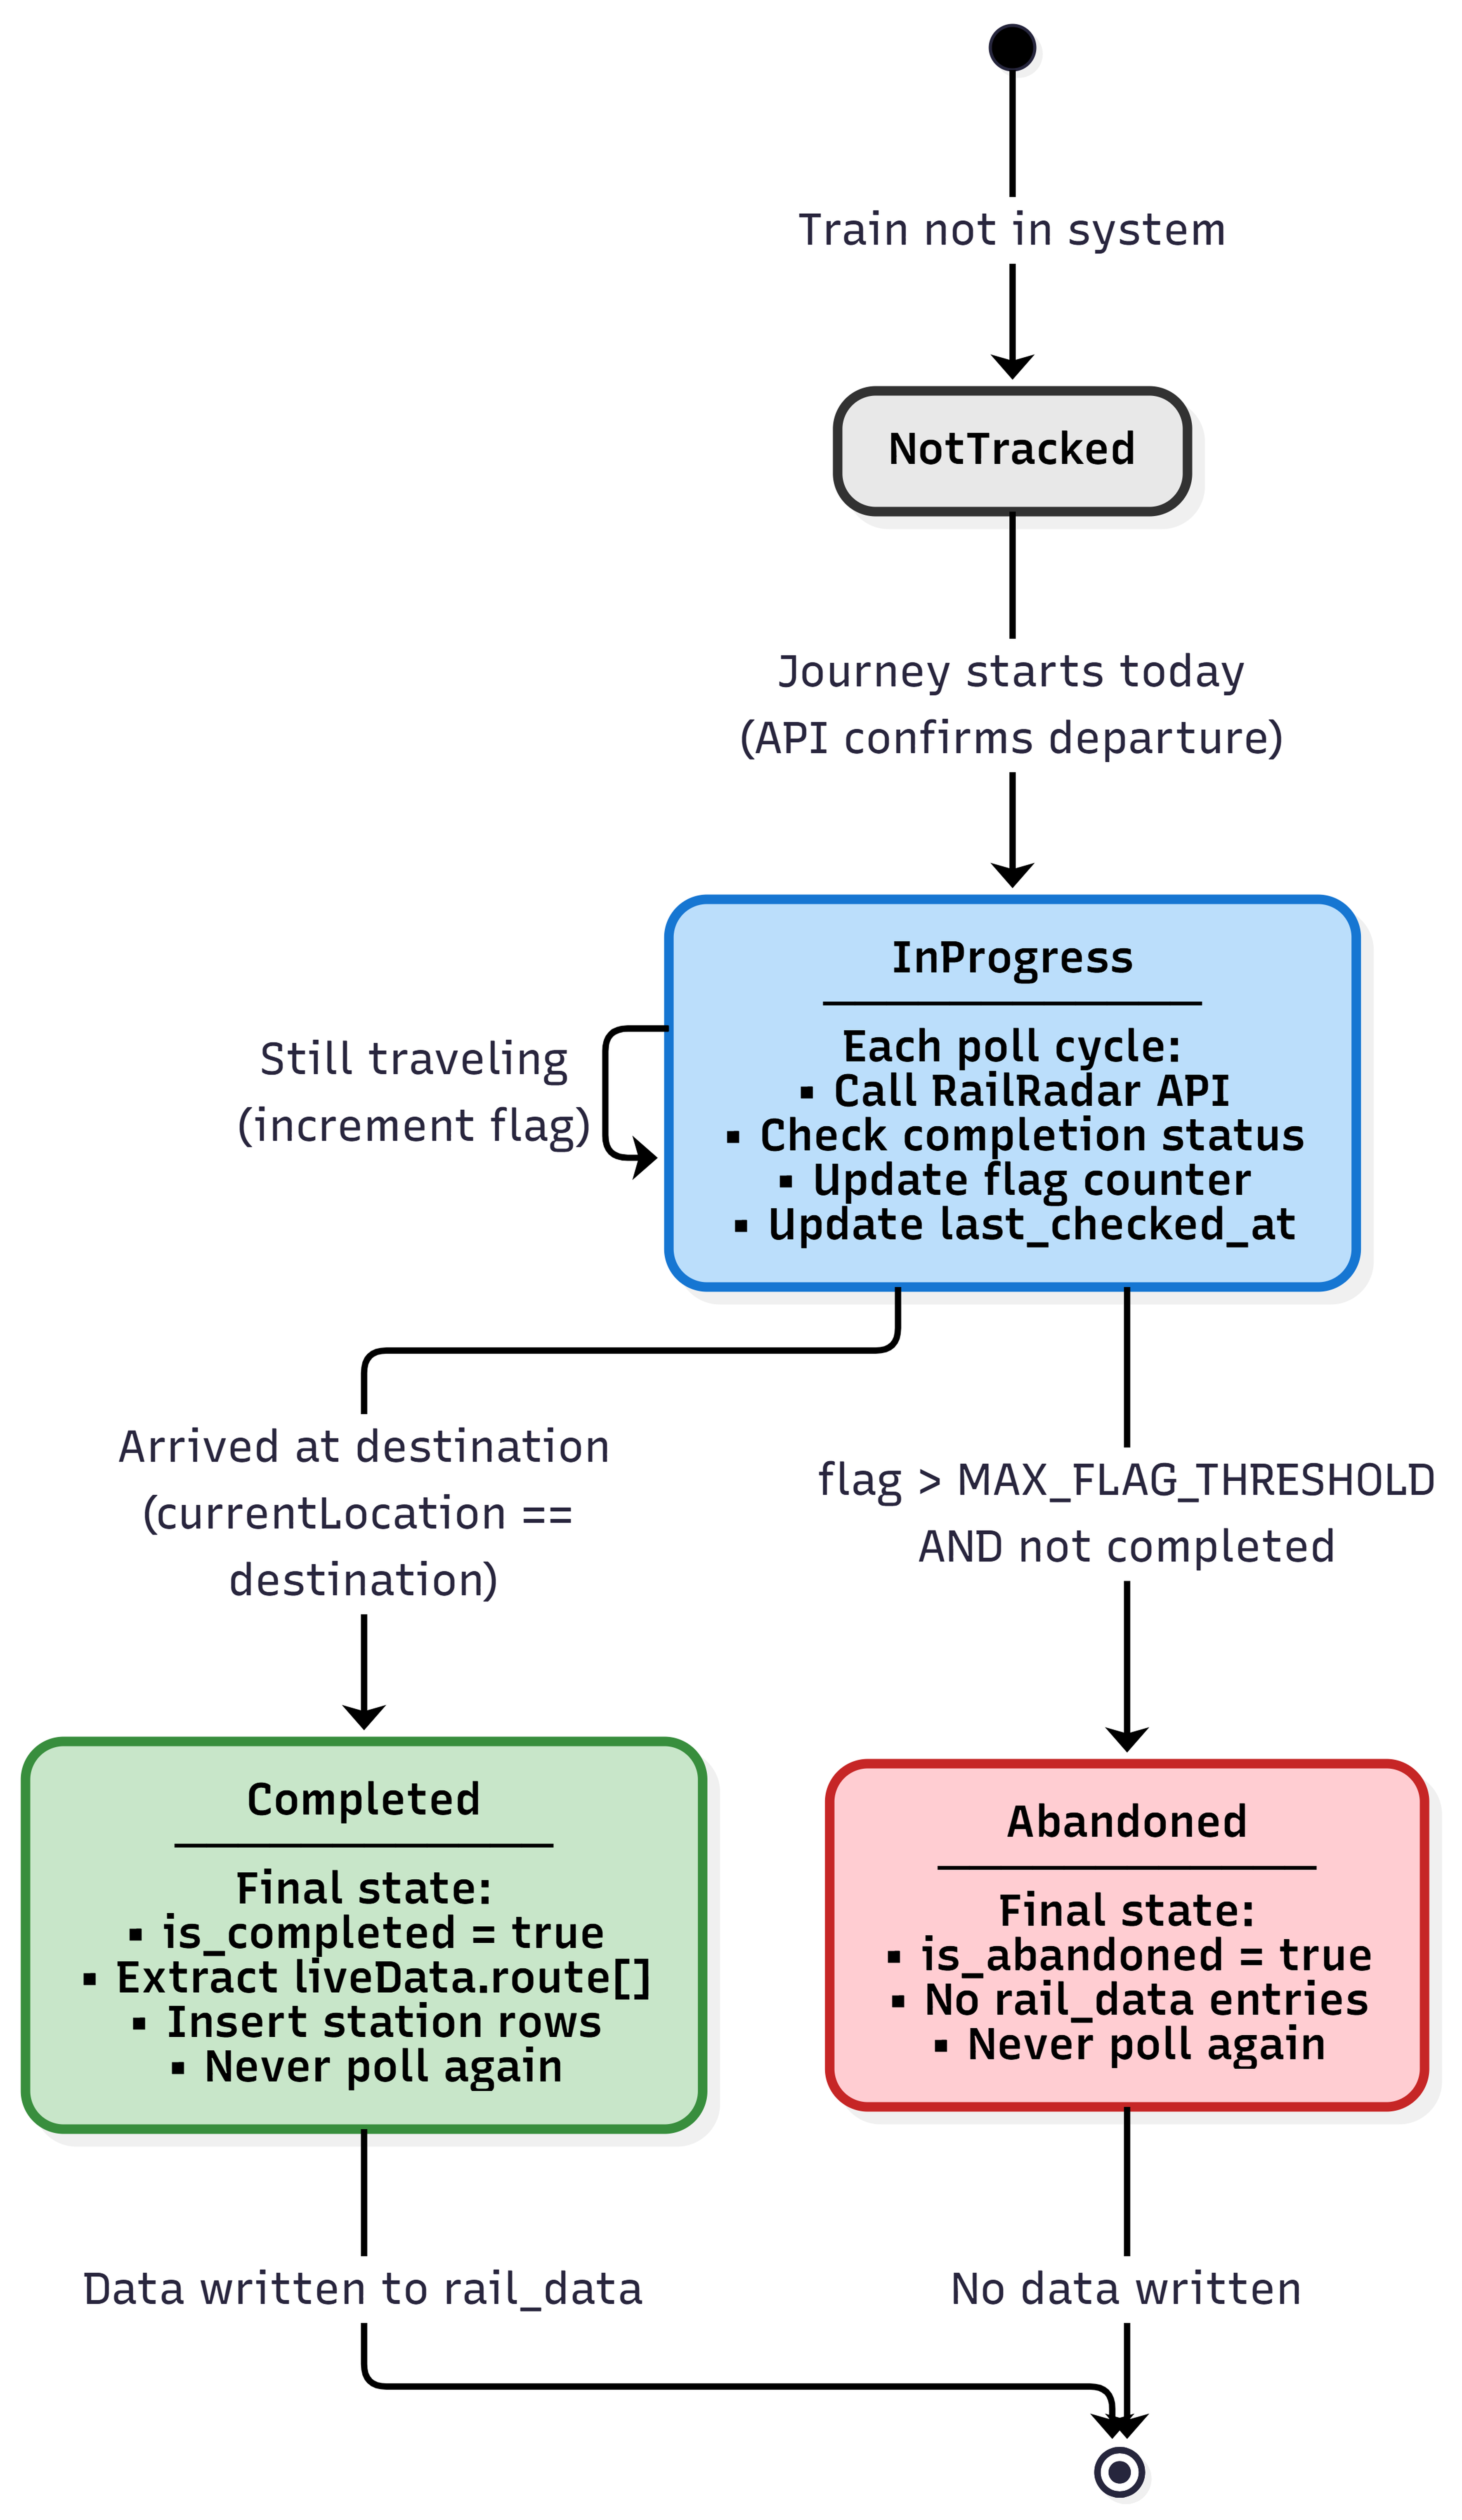
\includegraphics[width=\linewidth]{journey_state_diagram.png}
\caption{Journey state machine used for robust lifecycle tracking.}
\label{fig:state_machine}
\end{figure}

\subsection{Database design}
The data model consists of three connected tables. The \texttt{train\_info}
table stores static metadata for monitored trains, including train name,
journey type (single-day or multi-day), destination station code, and journey
duration. The \texttt{journey\_status\_flags} table tracks journey-level
state---completion, abandonment, and the polling flag count---keyed by a
unique combination of train number and journey date. The \texttt{rail\_data}
table stores station-level observations with scheduled and actual arrival and
departure timestamps and arrival and departure delay fields, keyed by train
number, journey date, and station code, and additionally records the distance
from origin in kilometers. Table~\ref{tab:db_schema} summarizes the tables,
their key fields, and their roles.

\begin{table}[width=\columnwidth,cols=1,pos=h]
\caption{Database schema summary.}
\label{tab:db_schema}
\setlength{\tabcolsep}{2.5pt}
\begin{tabular*}{\tblwidth}{@{\extracolsep{\fill}}p{0.19\linewidth}p{0.34\linewidth}p{0.39\linewidth}@{}}
\toprule
Table & Key fields & Role and important columns \\
\midrule
\texttt{train\_info} &
\texttt{train\_no} (unique) &
Static metadata: name, journey type, destination code, duration \\
\addlinespace
\texttt{journey\_\allowbreak status\_\allowbreak flags} &
\texttt{train\_no} $+$ \texttt{journey\_\allowbreak date} (unique) &
Journey state: flag count, completion and abandonment flags, check timestamps \\
\addlinespace
\texttt{rail\_data} &
\texttt{train\_no} $+$ \texttt{journey\_\allowbreak date} $+$ \texttt{station\_\allowbreak code} (unique) &
Station observations: scheduled and actual times, arrival and departure delay, distance from origin \\
\bottomrule
\end{tabular*}
\end{table}

\subsection{Reliability and data integrity}
Data reliability is maintained through four design decisions:
\begin{itemize}
    \item an idempotent insertion policy avoids duplicate station rows when
          the same journey is polled repeatedly;
    \item composite keys maintain journey isolation when multiple journeys
          are handled in parallel;
    \item API failures are handled through controlled flag increments rather
          than by corrupting existing state;
    \item completion detection and record insertion are logically tied
          together, so partially observed journeys cannot leave the dataset
          inconsistent.
\end{itemize}
Idempotency is the property that matters most in continuous polling, because
a station's record may legitimately be observed several times before
departure delay is finalized. By keying insertions on the journey and station
identity, repeated observation refreshes the same row instead of appending
duplicates, so record counts remain meaningful as a measure of collection
volume.

\subsection{Train panel and collection scope}
Ten representative trains were selected for continuous monitoring: four
single-day services and six multi-day services, spanning short commuter routes
and long-distance corridors. This mix was chosen deliberately so that the
dataset covers both rapid, high-frequency services and journeys long enough
to exhibit multi-stage delay accumulation. Table~\ref{tab:trains} lists the
monitored panel.

\begin{table}[width=\columnwidth,cols=4,pos=h]
\caption{Monitored train panel used in the current phase.}
\label{tab:trains}
\setlength{\tabcolsep}{3.2pt}
\begin{tabular*}{\tblwidth}{@{\extracolsep{\fill}}l l l l@{}}
\toprule
Train no. & Train name & Type & Dur. (h) \\
\midrule
61631  & Bhopal--Bina MEMU        & one-day   & 3 \\
11605  & Bhopal--Bina MEMU Exp.   & one-day   & 2 \\
11606  & Bina--Bhopal MEMU Exp.   & one-day   & 2 \\
61632  & Bina--Bhopal MEMU        & one-day   & 3 \\
12137  & Punjab Mail              & multi-day & 33 \\
12138  & Punjab Mail              & multi-day & 33 \\
11077  & Jhelum Express           & multi-day & 40 \\
11078  & Jhelum Express           & multi-day & 40 \\
18237  & Chhattisgarh Express     & multi-day & 43 \\
18238  & Chhattisgarh Express     & multi-day & 42 \\
\bottomrule
\end{tabular*}
\end{table}

\subsection{Delay variables and journey representation}
Two primary variables are used throughout the analysis: delay at arrival and
delay at departure, both measured in minutes. These are combined with the
scheduled and actual timestamps at each station, which allows delay
accumulation and recovery to be examined segment by segment rather than only
as an end-to-end figure.

Journey lifecycle tracking is treated as a first-class part of the data model
rather than as an afterthought. Instead of collecting raw snapshots alone,
each journey carries explicit completion and abandonment flags, which enables
controlled extraction of completed journeys and reduces duplication in
downstream analysis. This is what allows the analysis to state coverage
explicitly: a segment observed on 30 of 30 journey dates is quantitatively
different from one observed on 4 of 30.

Route analysis is performed on the halt-only station order. Using a single
static halt sequence for a train provides consistent sequence alignment across
different journey dates, so that any two journeys of the same train can be
compared position by position and segment-level differences can be attributed
to operational behavior rather than to changing station lists.

\subsection{Data processing and exploratory analysis workflow}
After the collection pipeline was established, a structured analysis phase was
executed in Python notebooks, in the following order:
\begin{enumerate}
    \item initial statistical exploratory analysis and data-quality checks,
          including column profiling, datatype checks, missing-value ratios,
          and timestamp parse diagnostics;
    \item time normalization and event-time construction, converting Unix
          timestamps to IST and deriving a consistent journey date for
          sequence analysis;
    \item train-wise delay-curve visualization, plotting station against
          departure delay across journey windows using the static
          halt-station ordering;
    \item pattern discovery, identifying visually that some station segments
          repeatedly add delay while others repeatedly cover up delay;
    \item baseline modeling, providing first benchmark models for delay
          forecasting using classical machine learning and time-series
          baselines;
    \item segment-level experimentation on Train 18238, computing
          station-pair delay deltas and alpha values and producing top-10
          rankings for delay-adding and delay-recovery pairs.
\end{enumerate}
Steps one and two are prerequisites rather than analysis: without consistent
time normalization, the same physical event can be assigned to different
journey dates, which silently corrupts every later comparison. Step three
produces the visual evidence on which the alpha hypothesis rests, and steps
five and six split the work into model-based and indicator-based tracks that
can be evaluated independently.

\subsubsection{From visualization to alpha experimentation}
The alpha methodology was derived directly from the observed shapes of the
station-wise delay trends. The analysis formalizes pairwise delay deltas,
computes the median and mean alpha, and reports ranked outputs, including the
top-10 delay-adding and top-10 recovery segments. Reporting both a ranked list
and an explicit coverage ratio for every pair keeps the interpretation
honest: a large alpha supported by only a few observations is visibly
distinguished from one supported by the full analysis window.

\subsection{Station-pair alpha metric}
To quantify station-segment behavior, $\alpha$ is defined on adjacent
halt-station pairs within a journey as the difference between the departure
delay recorded at the downstream station and the departure delay recorded at
the upstream station:
\begin{equation}
\alpha_{(i \rightarrow i+1)} = d_{i+1}^{(dep)} - d_i^{(dep)}
\label{eq:alpha}
\end{equation}
where $d_i^{(dep)}$ denotes the departure delay in minutes at station $i$. A
positive alpha indicates a delay-addition segment, a negative alpha indicates
a delay-recovery (cover-up) segment, and a practical threshold of
$|\alpha| \geq 1$ minute is applied to filter negligible fluctuations. Median
alpha across the observed journey dates is used as the primary robust
indicator, with mean alpha computed as a sensitivity check so that outlier
journeys cannot silently dominate the ranking.

The construction deliberately measures the difference between two adjacent
departure delays rather than an absolute delay value. This makes the
indicator independent of how delayed a journey already was when it reached the
upstream station, so a segment's tendency to add or absorb delay can be
compared across journeys with very different starting conditions.

\section{Experimental results and analysis}
\label{sec:results}

\subsection{Dataset snapshot and preprocessing}
The collection system ran from January to June 2026 and collected more than
61{,}000 unique station-level records. The data used for the visualizations
and modeling in this paper spans 1 January to 24 May 2026. For analysis,
timestamp fields were parsed and converted to IST, and both the journey date
and the halt-station sequence were normalized to support cross-journey
comparison. The primary fields used in this phase are train number, journey
date, station code, scheduled and actual arrival and departure timestamps,
arrival and departure delay, and the event-time-derived ordering used for
sequence construction.

The dataset therefore contains, for each completed journey of each monitored
train, an ordered sequence of halt stations with scheduled and actual times
and the corresponding delay values. Because insertion is idempotent and
completion is verified before insertion, the station-level record count is a
usable measure of collection volume rather than an inflated count of repeated
polling attempts.

Table~\ref{tab:dataset_stats} summarizes the dataset as evaluated for analysis
quality. The departure-delay distribution is strongly right-skewed (median
26 minutes, mean 44 minutes, 95th percentile 141 minutes), which motivates the
median-based aggregation used by the alpha metric and the choice of absolute
over percentage-based model errors. About 10\,\% of records lack a realized
departure time and about 4\,\% a realized arrival time at extraction; these
rows are removed by listwise deletion in the modeling stages, and the
distance-from-origin column is unpopulated throughout and therefore unused.

\begin{table}[width=\columnwidth,cols=2,pos=h]
\caption{Dataset evaluation summary.}
\label{tab:dataset_stats}
\begin{tabular*}{\tblwidth}{@{\extracolsep{\fill}}l r@{}}
\toprule
Statistic & Value \\
\midrule
Station-level records collected        & 61{,}169 \\
Records in analysis export            & 55{,}108 \\
Completed train journeys              & 1{,}243 \\
Journey dates (analysis export)       & 130 \\
Monitored trains                      & 10 \\
Distinct stations                     & 169 \\
Train 18238 records / journeys        & 9{,}095 / 107 \\
Missing departure delay (\%)          & 10.2 \\
Missing arrival delay (\%)            & 3.8 \\
Departure delay median / mean (min)   & 26.0 / 44.2 \\
Departure delay IQR (min)              & 13--53 \\
Departure delay 95th percentile (min) & 141 \\
\bottomrule
\end{tabular*}
\end{table}

\subsection{Train-wise delay pattern visualization}
For each train, a 30-day station-versus-departure-delay analysis was generated
in static, halt-only route order. Overlapping journey traces showed that route
behavior is not random: specific segments repeatedly exhibit upward delay drift
while others repeatedly reduce delay. Train 18238 (Chhattisgarh Express) is
presented here as the representative experimentation case, since it covers a
long multi-day corridor with sufficient journey repetitions in the analysis
window; corresponding results for the remaining nine trains are available from
the authors. Fig.~\ref{fig:train18238_delay} shows the resulting 30-day delay
pattern.

The visualization is intentionally diagnostic rather than predictive. By
overlaying journeys on a common station axis, it becomes possible to see
whether a vertical spread at a particular station reflects a consistent
segment effect or simply the accumulated delay of individual runs.

\begin{figure*}[width=\textwidth]
\centering
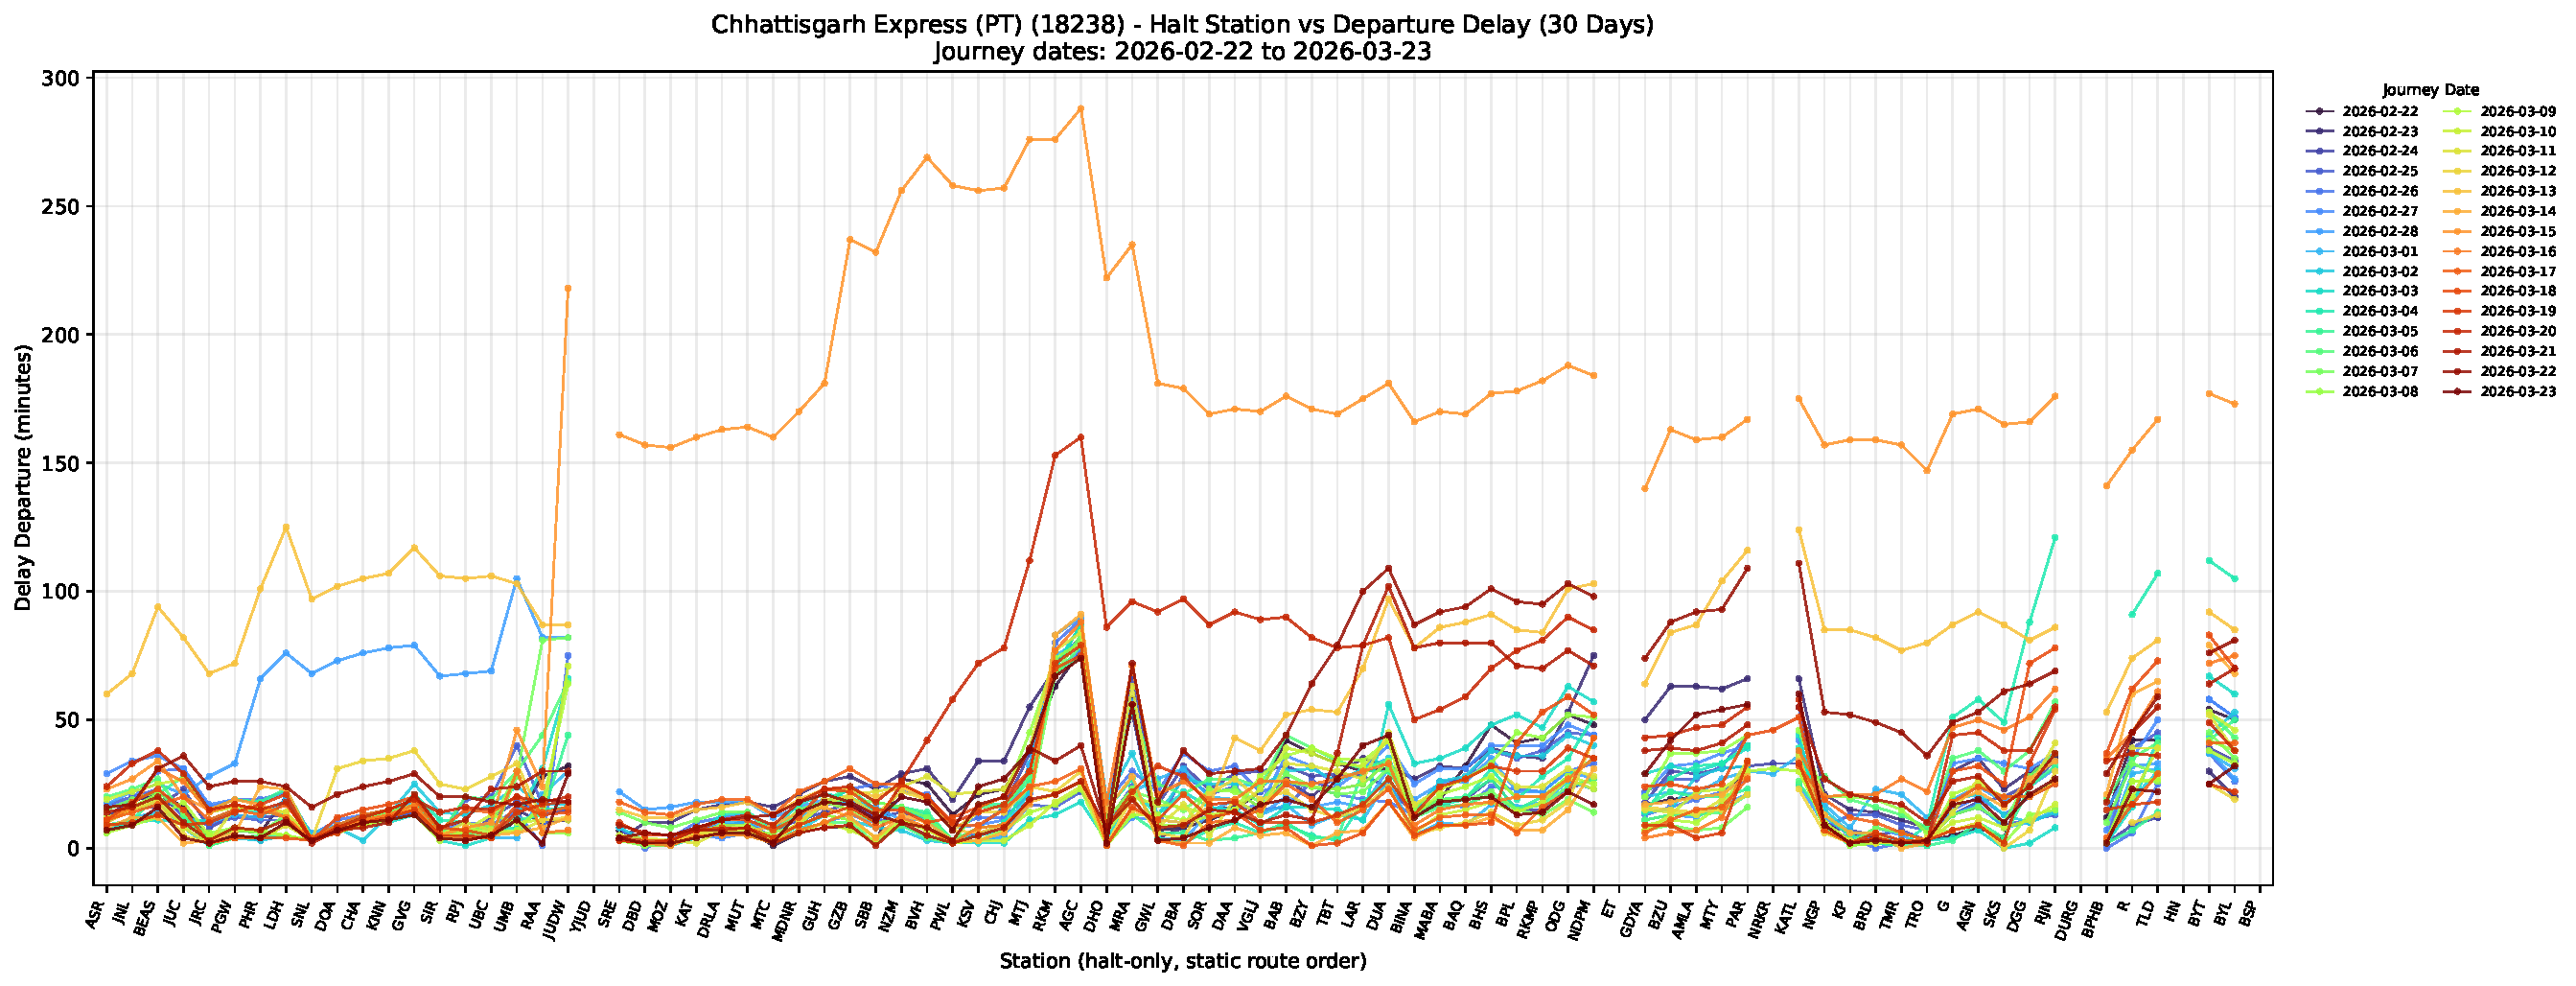
\includegraphics[width=\textwidth]{train_18238_station_delay_30d.pdf}
\caption{Train 18238 (Chhattisgarh Express): halt-station versus departure
delay pattern over the selected analysis window.}
\label{fig:train18238_delay}
\end{figure*}

\subsection{Station-pair alpha findings}
Applying the alpha metric of \eqref{eq:alpha} to Train 18238 over the 30-day
window shows that the route does not follow a single monotonic trend; it
alternates between delay-add and recovery zones. Representative delay-adding
segments include MTJ~$\rightarrow$~RKM, BPHB~$\rightarrow$~R, and
DHO~$\rightarrow$~MRA, while representative recovery segments include
AGC~$\rightarrow$~DHO, KATL~$\rightarrow$~NGP, and DUA~$\rightarrow$~BINA.
This supports the hypothesis that station and segment operational effects are
persistent and measurable. Fig.~\ref{fig:alpha_profile_18238} shows the
corresponding alpha profile for the route.

\begin{figure*}[width=\textwidth]
\centering
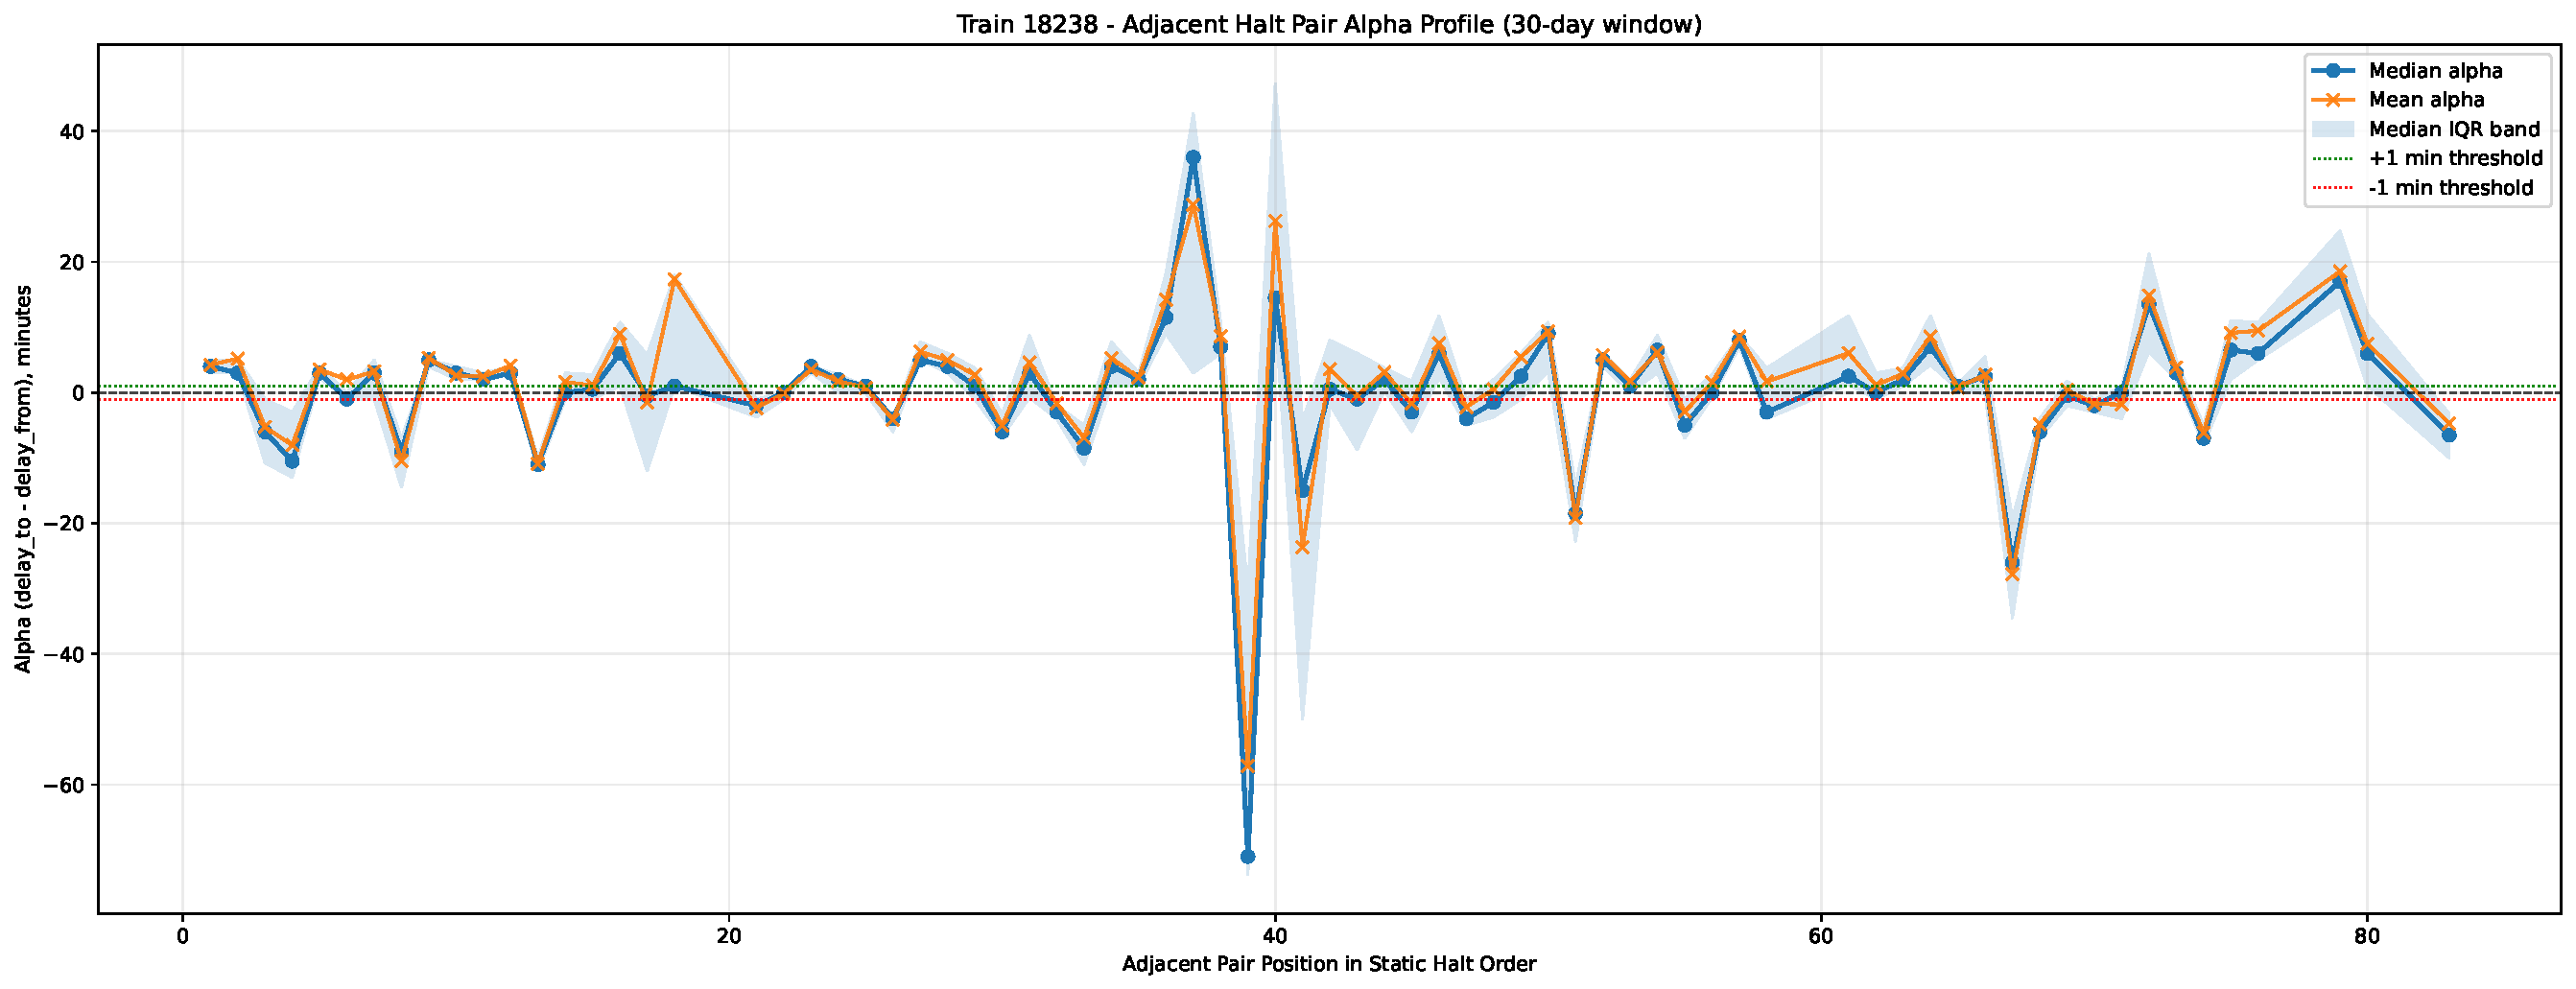
\includegraphics[width=\textwidth]{alpha_profile_plot.pdf}
\caption{Train 18238 adjacent halt-pair alpha profile for the selected 30-day
analysis window.}
\label{fig:alpha_profile_18238}
\end{figure*}

Table~\ref{tab:top_add} ranks the ten strongest delay-adding pairs by median
alpha, and Table~\ref{tab:top_cover} ranks the ten strongest recovery pairs.
The AGC~$\rightarrow$~DHO pair shows the largest median recovery
($-71.0$ minutes), while MTJ~$\rightarrow$~RKM shows the largest median
addition ($+36.0$ minutes). Both pairs were observed across all 30 sampled
journey dates ($n=30$), indicating full coverage and therefore low sampling
uncertainty for these estimates.

Two features of these rankings are operationally meaningful. First, the
largest effects are concentrated at a small number of route positions rather
than distributed evenly along the corridor, which suggests that improvement
efforts would be more effective if targeted at specific segments than if
applied uniformly. Second, additions and recoveries are interleaved along the
route: a corridor that appears severely delayed overall may still contain
segments that consistently absorb delay, and those segments are precisely
where the route's existing slack is being consumed.

\begin{table}[width=\columnwidth,cols=5,pos=h]
\caption{Top-10 delay-adding halt pairs by median $\alpha$ (Train 18238).}
\label{tab:top_add}
\setlength{\tabcolsep}{3.2pt}
\begin{tabular*}{\tblwidth}{@{\extracolsep{\fill}}l c c c c@{}}
\toprule
Pair & $n$ & Cov. & Med.\ $\alpha$ & Mean $\alpha$ \\
\midrule
MTJ $\rightarrow$ RKM & 30 & 1.000 &  36.000 &  28.733 \\
BPHB $\rightarrow$ R  & 26 & 0.867 &  17.000 &  18.538 \\
DHO $\rightarrow$ MRA & 30 & 1.000 &  14.500 &  26.267 \\
TRO $\rightarrow$ G    & 30 & 1.000 &  13.500 &  14.833 \\
CHJ $\rightarrow$ MTJ & 30 & 1.000 &  11.500 &  14.200 \\
LAR $\rightarrow$ DUA  & 30 & 1.000 &   9.000 &   9.367 \\
RKMP $\rightarrow$ ODG & 30 & 1.000 &   8.000 &   8.567 \\
RKM $\rightarrow$ AGC  & 30 & 1.000 &   7.000 &   8.600 \\
MTY $\rightarrow$ PAR  & 30 & 1.000 &   7.000 &   8.567 \\
SKS $\rightarrow$ DGG  & 30 & 1.000 &   6.500 &   9.133 \\
\bottomrule
\end{tabular*}
\end{table}

\begin{table}[width=\columnwidth,cols=5,pos=h]
\caption{Top-10 cover-up (recovery) halt pairs by median $\alpha$
(Train 18238).}
\label{tab:top_cover}
\setlength{\tabcolsep}{3.2pt}
\begin{tabular*}{\tblwidth}{@{\extracolsep{\fill}}l c c c c@{}}
\toprule
Pair & $n$ & Cov. & Med.\ $\alpha$ & Mean $\alpha$ \\
\midrule
AGC $\rightarrow$ DHO & 30 & 1.000 & $-71.000$ & $-57.167$ \\
KATL $\rightarrow$ NGP & 30 & 1.000 & $-26.000$ & $-27.800$ \\
DUA $\rightarrow$ BINA & 30 & 1.000 & $-18.500$ & $-19.167$ \\
MRA $\rightarrow$ GWL & 30 & 1.000 & $-15.000$ & $-23.633$ \\
GVG $\rightarrow$ SIR & 30 & 1.000 & $-11.000$ & $-10.900$ \\
JUC $\rightarrow$ JRC  & 30 & 1.000 & $-10.500$ &  $-8.033$ \\
LDH $\rightarrow$ SNL & 30 & 1.000 &  $-9.000$ & $-10.500$ \\
BVH $\rightarrow$ PWL & 30 & 1.000 &  $-8.500$ &  $-6.933$ \\
AGN $\rightarrow$ SKS & 30 & 1.000 &  $-7.000$ &  $-6.133$ \\
BYT $\rightarrow$ BYL & 30 & 1.000 &  $-6.500$ &  $-4.733$ \\
\bottomrule
\end{tabular*}
\end{table}

The mean-alpha sensitivity check yields a largely overlapping ranking:
RAA~$\rightarrow$~JUDW, DGG~$\rightarrow$~RJN, and UBC~$\rightarrow$~UMB
enter the top-10 delay-adding list in place of RKMP~$\rightarrow$~ODG,
RKM~$\rightarrow$~AGC, and MTY~$\rightarrow$~PAR, while
BEAS~$\rightarrow$~JUC enters and BYT~$\rightarrow$~BYL leaves the cover-up
list under the mean criterion; the dominant pairs retain their positions at
the top. This indicates that the identified segments are not artifacts of a
single aggregation choice. The full mean-based rankings and the route-ordered
alpha profile for the whole route are reproduced in Appendix~\ref{app:alpha}
and Appendix~\ref{app:mean}, where the coverage ratio is reported alongside
median and mean values for every adjacent halt pair.

Low-coverage pairs were mainly concentrated around sparse route segments (for
example PAR~$\rightarrow$~NRKR and NRKR~$\rightarrow$~KATL, each observed on
only 4 of 30 dates, with a coverage ratio of 0.133), while several downstream
pairs had no observations in the selected 30-day window. These estimates
should therefore be treated as provisional until additional journey data are
collected, and they are reported here for completeness rather than as
established segment behavior. The same caution applies to
BPHB~$\rightarrow$~R in Table~\ref{tab:top_add}, whose coverage of 0.867
reflects 26 of 30 dates rather than the full window.

\subsection{Baseline modeling and evaluation}
Baseline next-station delay prediction was performed with a journey-wise split
to reduce leakage between training and evaluation. Splitting by journey rather
than by row ensures that observations from the same run do not appear on both
sides of the split, which would otherwise inflate apparent accuracy because
consecutive stations of one journey are strongly correlated; concretely, the
latest 20\,\% of journey dates are held out as the test set. Initial
supervised models (random forest \citep{breiman2001random} and polynomial
regression) were fit on Train 11077 over the January--March extract of the
collection, while the main modeling effort targeted Train 18238 over the
analysis window of 1 January to 24 May 2026 and added statistical baselines,
tuned gradient boosting, and sequence models. Table~\ref{tab:model_metrics}
reports the resulting evaluation; the sequence models are scored over sliding
windows of the same held-out journeys.

\begin{table}[width=\columnwidth,cols=4,pos=h]
\caption{Model evaluation on held-out test journeys (MAE and RMSE in minutes).}
\label{tab:model_metrics}
\setlength{\tabcolsep}{3.6pt}
\begin{tabular*}{\tblwidth}{@{\extracolsep{\fill}}l l c c@{}}
\toprule
Model & Train & MAE & RMSE \\
\midrule
TCN & 18238 & \textbf{4.778} & \textbf{8.105} \\
LSTM & 18238 & 4.988 & 8.634 \\
XGBoost (tuned) & 18238 & 5.532 & 8.234 \\
Linear regression & 18238 & 7.160 & 10.277 \\
Ridge regression & 18238 & 7.161 & 10.275 \\
Persistence (naive) & 18238 & 8.375 & 14.190 \\
Rolling mean (3) & 18238 & 12.257 & 17.100 \\
\midrule
Random forest & 11077 & 11.592 & 18.534 \\
Polynomial regression & 11077 & 12.322 & 19.082 \\
\bottomrule
\end{tabular*}
\end{table}

Three findings are notable. First, the naive persistence baseline, which
repeats the currently observed delay as the next-station prediction, already
reaches a MAE of 8.375 minutes; the random forest (11.592), polynomial
regression (12.322), and rolling-mean (12.257) baselines fail to beat it,
while linear and ridge regression improve on it only marginally (about
7.2 minutes), so the added model complexity in those baselines is not yet
paying off. Second, the tuned XGBoost model (5.532) and the sequence models do
clear the bar, with the TCN achieving the best result overall (MAE 4.778,
RMSE 8.105), about 43\,\% lower MAE than persistence; error analysis of the
tuned XGBoost model shows a MAE of 5.485 minutes on overnight segments against
6.247 minutes during the day, and a recursive multi-station rollout on a
sample test journey degrades to a MAE of 11.273 minutes as predictions are fed
back as inputs. Third, percentage-based error remains unusable for this
target: the mean absolute percentage error (MAPE) for the initial baselines is
on the order of $10^{6}$ percent ($5.26\times10^{6}$ for the random forest and
$3.25\times10^{6}$ for polynomial regression), reflecting instability near
zero-delay denominators, so absolute error measures are treated as the
meaningful indicators. Even the best current results are not yet sufficient to
capture all learned route-level patterns, which is consistent with the finding
that delay behavior is strongly segment-dependent and therefore not fully
described by the features used so far.

\subsubsection{Time-series trials}
ARIMA and SARIMA \citep{boxjenkins1976}, Prophet \citep{taylor2018forecasting},
and Chronos \citep{woo2024chronos} baselines were explored, but their initial
outcomes were not adequate for the desired route-pattern capture. The current
phase therefore treats these as reference baselines rather than final
predictive claims, and they are retained to document which model families were
assessed before the next phase of feature engineering. A plausible reason for
their limited performance at this stage is that the series available per train
and per station are still short, so classical time-series models have too
little history to estimate stable seasonal components.

\subsection{Comparison with prior work}
A direct numeric ranking against the literature is not meaningful because the
closest studies target different quantities, so Table~\ref{tab:prior_comparison}
states each study's target explicitly alongside its reported values and our
corresponding result.

\begin{table*}[width=\textwidth]
\caption{Comparison with prior work. Values are as reported in each study;
our results are those of Table~\ref{tab:model_metrics}.}
\label{tab:prior_comparison}
\setlength{\tabcolsep}{3pt}
\renewcommand{\arraystretch}{0.92}
\begin{tabular*}{\tblwidth}{@{\extracolsep{\fill}}p{0.135\textwidth}p{0.150\textwidth}p{0.185\textwidth}p{0.135\textwidth}p{0.175\textwidth}p{0.120\textwidth}@{}}
\toprule
Study & Scope & Task / target & Metric & Reported result & Our result \\
\midrule
Gaurav \& Srivastava \citep{gaurav2018zeroshot} &
135 trains via Mughalsarai, 2016--2018 &
Arrival late-minutes at in-line stations (feed-forward) &
95\,\% CI coverage; per-journey RMSE (min) &
Coverage 62.5\,\% (known) / 15.0\,\% (zero-shot); RMSE 11.8--96.6 &
RMSE \textbf{8.1} (TCN) \\
\addlinespace
Arshad \& Ahmed \citep{arshad2019prediction} &
Indian Railways survey and proposed protocol &
Multivariate regression, neural networks, and random forest compared for delay prediction &
Accuracy; training time &
No numeric results reported &
MAE \textbf{4.8} / RMSE \textbf{8.1} \\
\addlinespace
Chowdhury et al.\ (RSTGCN) \citep{chowdhury2025rstgcn} &
Whole IRN, 4{,}735 stations, Sep.\ 2024 &
Station-hourly average arrival delay, 1\,h horizon &
MAE (h), MAPE (\%), RMSE (h) &
MAE 0.075\,h ($\approx$4.5\,min); MAPE 9.2\,\%; RMSE $\approx$22.8\,min &
MAE \textbf{4.8}\,min \\
\bottomrule
\end{tabular*}
\end{table*}

Gaurav and Srivastava predict arrival late-minutes with feed-forward models
and report per-journey RMSE of 11.8--96.6\,min, with 95\,\% interval coverage
falling from about 62.5\,\% on known trains to about 15.0\,\% in their
zero-shot setting \citep{gaurav2018zeroshot}; our TCN attains an RMSE of
8.1\,min on next-station departure delay under a chronological journey-wise
split, a tighter target that is not directly rankable against theirs. Arshad
and Ahmed propose comparing multivariate regression, neural networks, and
random forest for Indian delay prediction but report no numeric results
\citep{arshad2019prediction}. RSTGCN predicts station-level hourly average
arrival delay over 4{,}735 stations, reporting an MAE of 0.075\,h
(4.5\,min) and MAPE of 9.2\,\% \citep{chowdhury2025rstgcn}; our per-train MAE
of 4.8\,min is of similar magnitude, although our target is a single train's
departure delay rather than a spatial average, while RSTGCN's RMSE of about
22.8\,min is far larger than our 8.1\,min, reflecting the heavier tail of
station-wide aggregates. Oneto et al., Flier et al., and Goverde
\citep{oneto2018train,flier2009delay,goverde2010railway} address delay
distribution and propagation rather than point-forecast accuracy and are
therefore compared only qualitatively. Consistent with RSTGCN's practice of
treating zero actual delay explicitly when computing percentage error
\citep{chowdhury2025rstgcn}, we also report MAPE with caution because
near-zero delays make it unstable in our setting.

\subsection{Limitations in the current experimental phase}
The present results are subject to the following limitations:
\begin{itemize}
    \item selection bias can occur when severely delayed journeys cross the
          abandonment thresholds and are therefore excluded from the
          completed-journey dataset;
    \item coverage is currently limited to about four and a half months of
          continuous data across ten trains (January--June 2026), so
          network-wide generalization is pending;
    \item exogenous-factor comparison is limited: this phase did not observe
          strong seasonal extremes such as severe fog or monsoon rain, so
          weather-impact learning is weak in the present baselines;
    \item experiments are primarily single-source and do not yet integrate
          richer factors such as weather feeds, infrastructure constraints,
          or control actions;
    \item baseline models do not yet fully encode station-network structure,
          so interactions between neighboring segments remain implicit;
    \item congestion attribution is limited: alpha locates persistent
          delay-adding zones from single-train traces, but confirming
          station congestion requires concurrent multi-train observations
          at shared stations, which is deferred to future work.
\end{itemize}
The first two limitations interact: if severely delayed journeys are more
likely to be abandoned, and abandonment is more likely during disruptive
periods, then the retained dataset is progressively biased toward undisturbed
operations. This is one reason the alpha results are presented as segment
tendencies with explicit coverage rather than as unconditional delay
estimates. Data collection was paused on 8 June 2026, so observations are not available after that date.

\section{Conclusion and future work}
\label{sec:conclusion}

\subsection{Conclusion}
This work established a data-centric pipeline for Indian Railways delay
analytics and demonstrated that reliable station-level data generation is
feasible with automated cloud workflows. It has produced:
\begin{itemize}
    \item a running collection infrastructure that requires no manual
          intervention;
    \item a real-time dataset of more than 61{,}000 station-level records
          collected January--June 2026;
    \item interpretable route-segment findings obtained through the alpha
          analysis; and
    \item reproducible baseline modeling benchmarks for next-station delay
          prediction.
\end{itemize}
The core academic contribution of this phase is not a final high-accuracy
predictor, but a robust and transparent data foundation together with
interpretable diagnostics that make future modeling meaningful in a domain
where operational variability is high and open data are scarce. Because the
pipeline and the analysis both operate on explicit, traceable records,
subsequent modeling work can be compared on a common and reproducible basis.
The alpha results in particular turn the dataset into an operational
diagnostic: they identify which segments consistently consume recovery margin
and which consistently provide it, information that is useful even before a
predictive model is deployed.

\subsection{Future work}
Planned next steps are:
\begin{enumerate}
    \item advanced preprocessing and normalization of delay and time features;
    \item station-network-aware feature engineering;
    \item graph-based representations for delay propagation;
    \item improved objective functions and robust evaluation metrics beyond
          MAPE;
    \item scaling train coverage and extending the collection horizon to
          enable concurrent-station analysis, where all trains sharing a
          station are observed together to confirm congestion effects.
\end{enumerate}

A particularly promising direction is graph-embedding-based station-delay
prediction, as reported in recent literature \citep{chowdhury2025rstgcn}. This
aligns with our observation that delay behavior is strongly segment-dependent
and that the alpha indicator already exposes persistent structure which
network-aware models should be able to exploit.

\section*{Declaration of competing interest}

The authors declare that they have no known competing interests.

\section*{Funding}

This research did not receive any specific grant from funding agencies in the
public, commercial, or not-for-profit sectors.

\section*{Declaration of generative AI and AI-assisted technologies in the manuscript preparation process}

During the preparation of this work the author(s) used generative AI tools to
rephrase and restructure the manuscript and to correct LaTeX source errors. The
authors reviewed and edited all such content and take full responsibility for
the content of the published article.

\section*{Data availability}

The station-level delay dataset collected in this study is available on
reasonable request through \url{https://forms.gle/5JM1UZqLPvYseyuUA}.
Requests are handled by the corresponding author. The collection pipeline,
polling scripts, database schema, and analysis notebooks underlying the
reported results form part of the accompanying research record and can be
shared subject to the terms of the RailRadar application programming
interface.

\appendix

\section{Route-ordered alpha profile for Train 18238}
\label{app:alpha}

Table~\ref{tab:route_alpha} reports the route-ordered alpha profile for Train
18238 over the 30-day analysis window. Each row corresponds to an adjacent
halt pair, listed in route sequence, with the number of observed journeys, the
coverage ratio, and the median and mean alpha values. Route positions that were
not observed in the window are absent from the table, and the low-coverage
positions discussed in Section~\ref{sec:results} appear near route
position~65. Because the profile is too long for a single page, it is set as
two consecutive parts that form one continuous table: the first part carries
route positions 1--33 and the second continues with positions 34--83, with the
sequence numbering running unbroken across the page break.

\makeatletter
\def\@dbflt#1{\@ifnextchar[{\@xdblfloat{#1}}{\@xdblfloat{#1}[b]}}
\makeatother
\begin{table*}[width=\textwidth,pos=b]
\caption{Route-ordered alpha profile for Train 18238 (median and mean with
coverage ratio).}
\label{tab:route_alpha}
\setlength{\tabcolsep}{4pt}
\renewcommand{\arraystretch}{0.92}
\begin{tabular*}{\tblwidth}{@{\extracolsep{\fill}}r l c c c c@{}}
\toprule
Seq & Pair & $n$ & Cov. & Med.\ $\alpha$ & Mean $\alpha$ \\
\midrule
1  & ASR $\to$ JNL  & 30 & 1.000 &   4.000 &   4.233 \\
2  & JNL $\to$ BEAS & 30 & 1.000 &   3.000 &   5.200 \\
3  & BEAS $\to$ JUC & 30 & 1.000 &  $-6.000$ &  $-5.267$ \\
4  & JUC $\to$ JRC  & 30 & 1.000 & $-10.500$ &  $-8.033$ \\
5  & JRC $\to$ PGW  & 30 & 1.000 &   3.000 &   3.533 \\
6  & PGW $\to$ PHR  & 30 & 1.000 &  $-1.000$ &   1.967 \\
7  & PHR $\to$ LDH  & 30 & 1.000 &   3.000 &   3.233 \\
8  & LDH $\to$ SNL  & 30 & 1.000 &  $-9.000$ & $-10.500$ \\
9  & SNL $\to$ DOA  & 30 & 1.000 &   5.000 &   5.300 \\
10 & DOA $\to$ CHA  & 30 & 1.000 &   3.000 &   2.633 \\
11 & CHA $\to$ KNN  & 30 & 1.000 &   2.000 &   2.467 \\
12 & KNN $\to$ GVG  & 30 & 1.000 &   3.000 &   4.133 \\
13 & GVG $\to$ SIR  & 30 & 1.000 & $-11.000$ & $-10.900$ \\
14 & SIR $\to$ RPJ  & 30 & 1.000 &   0.000 &   1.633 \\
15 & RPJ $\to$ UBC  & 30 & 1.000 &   0.500 &   1.067 \\
16 & UBC $\to$ UMB  & 30 & 1.000 &   6.000 &   8.967 \\
17 & UMB $\to$ RAA  & 30 & 1.000 &  $-0.500$ &  $-1.500$ \\
18 & RAA $\to$ JUDW & 30 & 1.000 &   1.000 &  17.333 \\
21 & SRE $\to$ DBD  & 30 & 1.000 &  $-2.000$ &  $-2.333$ \\
22 & DBD $\to$ MOZ  & 30 & 1.000 &   0.000 &  $-0.133$ \\
23 & MOZ $\to$ KAT  & 30 & 1.000 &   4.000 &   3.533 \\
24 & KAT $\to$ DRLA & 30 & 1.000 &   2.000 &   1.733 \\
25 & DRLA $\to$ MUT & 30 & 1.000 &   1.000 &   0.733 \\
26 & MUT $\to$ MTC  & 30 & 1.000 &  $-4.000$ &  $-4.133$ \\
27 & MTC $\to$ MDNR & 30 & 1.000 &   5.000 &   6.267 \\
28 & MDNR $\to$ GUH & 30 & 1.000 &   4.000 &   4.933 \\
29 & GUH $\to$ GZB  & 30 & 1.000 &   1.000 &   2.733 \\
30 & GZB $\to$ SBB  & 30 & 1.000 &  $-6.000$ &  $-5.033$ \\
31 & SBB $\to$ NZM  & 30 & 1.000 &   3.000 &   4.600 \\
32 & NZM $\to$ BVH  & 30 & 1.000 &  $-3.000$ &  $-1.633$ \\
33 & BVH $\to$ PWL  & 30 & 1.000 &  $-8.500$ &  $-6.933$ \\
\midrule
\end{tabular*}
\end{table*}
\makeatletter
\def\@dbflt#1{\@ifnextchar[{\@xdblfloat{#1}}{\@xdblfloat{#1}[tp]}}
\makeatother

\begingroup
\makeatletter
\addtocounter{table}{-1}
\renewcommand{\thetable}{8 (continued)}
\makeatother
\begin{table*}[width=\textwidth,pos=t]
\caption{Route-ordered alpha profile for Train 18238 (median and mean with
coverage ratio), route positions 34--83.}
\setlength{\tabcolsep}{4pt}
\renewcommand{\arraystretch}{0.92}
\begin{tabular*}{\tblwidth}{@{\extracolsep{\fill}}r l c c c c@{}}
\toprule
Seq & Pair & $n$ & Cov. & Med.\ $\alpha$ & Mean $\alpha$ \\
\midrule
34 & PWL $\to$ KSV & 30 & 1.000 &   4.000 &   5.267 \\
35 & KSV $\to$ CHJ & 30 & 1.000 &   2.000 &   2.300 \\
36 & CHJ $\to$ MTJ & 30 & 1.000 &  11.500 &  14.200 \\
37 & MTJ $\to$ RKM & 30 & 1.000 &  36.000 &  28.733 \\
38 & RKM $\to$ AGC & 30 & 1.000 &   7.000 &   8.600 \\
39 & AGC $\to$ DHO & 30 & 1.000 & $-71.000$ & $-57.167$ \\
40 & DHO $\to$ MRA & 30 & 1.000 &  14.500 &  26.267 \\
41 & MRA $\to$ GWL & 30 & 1.000 & $-15.000$ & $-23.633$ \\
42 & GWL $\to$ DBA & 30 & 1.000 &   0.500 &   3.567 \\
43 & DBA $\to$ SOR & 30 & 1.000 &  $-1.000$ &  $-0.500$ \\
44 & SOR $\to$ DAA & 30 & 1.000 &   2.000 &   3.133 \\
45 & DAA $\to$ VGLJ & 30 & 1.000 &  $-3.000$ &  $-1.700$ \\
46 & VGLJ $\to$ BAB & 30 & 1.000 &   6.000 &   7.567 \\
47 & BAB $\to$ BZY & 30 & 1.000 &  $-4.000$ &  $-2.200$ \\
48 & BZY $\to$ TBT & 30 & 1.000 &  $-1.500$ &   0.500 \\
49 & TBT $\to$ LAR & 30 & 1.000 &   2.500 &   5.433 \\
50 & LAR $\to$ DUA & 30 & 1.000 &   9.000 &   9.367 \\
51 & DUA $\to$ BINA & 30 & 1.000 & $-18.500$ & $-19.167$ \\
52 & BINA $\to$ MABA & 30 & 1.000 &   5.000 &   5.733 \\
53 & MABA $\to$ BAQ & 30 & 1.000 &   1.000 &   1.733 \\
54 & BAQ $\to$ BHS & 30 & 1.000 &   6.500 &   6.133 \\
55 & BHS $\to$ BPL & 30 & 1.000 &  $-5.000$ &  $-2.933$ \\
56 & BPL $\to$ RKMP & 30 & 1.000 &   0.000 &   1.533 \\
57 & RKMP $\to$ ODG & 30 & 1.000 &   8.000 &   8.567 \\
58 & ODG $\to$ NDPM & 30 & 1.000 &  $-3.000$ &   1.667 \\
61 & GDYA $\to$ BZU & 30 & 1.000 &   2.500 &   6.033 \\
62 & BZU $\to$ AMLA & 30 & 1.000 &   0.000 &   1.167 \\
63 & AMLA $\to$ MTY & 30 & 1.000 &   2.000 &   2.867 \\
64 & MTY $\to$ PAR & 30 & 1.000 &   7.000 &   8.567 \\
65 & PAR $\to$ NRKR &  4 & 0.133 &   1.000 &   0.750 \\
66 & NRKR $\to$ KATL &  4 & 0.133 &   2.500 &   2.750 \\
67 & KATL $\to$ NGP & 30 & 1.000 & $-26.000$ & $-27.800$ \\
68 & NGP $\to$ KP   & 30 & 1.000 &  $-6.000$ &  $-4.867$ \\
69 & KP $\to$ BRD   & 30 & 1.000 &  $-0.500$ &   0.367 \\
70 & BRD $\to$ TMR  & 30 & 1.000 &  $-2.000$ &  $-1.733$ \\
71 & TMR $\to$ TRO  & 30 & 1.000 &   0.000 &  $-1.833$ \\
72 & TRO $\to$ G    & 30 & 1.000 &  13.500 &  14.833 \\
73 & G $\to$ AGN    & 30 & 1.000 &   3.000 &   3.833 \\
74 & AGN $\to$ SKS  & 30 & 1.000 &  $-7.000$ &  $-6.133$ \\
75 & SKS $\to$ DGG  & 30 & 1.000 &   6.500 &   9.133 \\
76 & DGG $\to$ RJN  & 30 & 1.000 &   6.000 &   9.467 \\
79 & BPHB $\to$ R   & 26 & 0.867 &  17.000 &  18.538 \\
80 & R $\to$ TLD    & 29 & 0.967 &   6.000 &   7.517 \\
83 & BYT $\to$ BYL  & 30 & 1.000 &  $-6.500$ &  $-4.733$ \\
\bottomrule
\end{tabular*}
\end{table*}
\endgroup

\section{Mean-alpha ranking tables}
\label{app:mean}

Table~\ref{tab:mean_add} reproduces the top-10 delay-adding pairs (left columns)
and the top-10 cover-up pairs (right columns) ranked by mean alpha, serving as
the sensitivity check for the median-based rankings reported in
Section~\ref{sec:results}; the route-ordered alpha profile is given in
Table~\ref{tab:route_alpha}. The interquartile range (IQR) of alpha is included
to indicate the spread of each pair across journey dates.

The two panels also illustrate where the mean and median diverge, which is
diagnostically informative. RAA~$\rightarrow$~JUDW, for example, enters the
mean-based delay-adding list with a mean alpha of 17.3 minutes while its
median is only 1.0 minute, indicating that a small number of outlier journeys
dominate its aggregate behavior. By contrast, pairs such as
MTJ~$\rightarrow$~RKM and AGC~$\rightarrow$~DHO show consistent median and mean
values of the same sign, which supports treating them as genuinely persistent
segment effects rather than artifacts of a few extreme runs.

\begin{table*}[width=\textwidth]
\caption{Top-10 rankings by mean alpha (Train 18238): delay-adding (left) and
cover-up (right).}
\label{tab:mean_add}
\setlength{\tabcolsep}{3.2pt}
\renewcommand{\arraystretch}{0.9}
\begin{tabular*}{\tblwidth}{@{\extracolsep{\fill}}l c c c c c@{\hspace{1.2em}}l c c c c c@{}}
\toprule
Pair & $n$ & Cov. & Med.\ $\alpha$ & Mean $\alpha$ & IQR &
Pair & $n$ & Cov. & Med.\ $\alpha$ & Mean $\alpha$ & IQR \\
\midrule
MTJ $\to$ RKM & 30 & 1.000 &  36.000 & 28.733 & 39.750 &
AGC $\to$ DHO & 30 & 1.000 & $-71.000$ & $-57.167$ & 43.750 \\
DHO $\to$ MRA & 30 & 1.000 &  14.500 & 26.267 & 35.000 &
KATL $\to$ NGP & 30 & 1.000 & $-26.000$ & $-27.800$ & 15.250 \\
BPHB $\to$ R & 26 & 0.867 &  17.000 & 18.538 & 11.500 &
MRA $\to$ GWL & 30 & 1.000 & $-15.000$ & $-23.633$ & 45.750 \\
RAA $\to$ JUDW & 30 & 1.000 &   1.000 & 17.333 & 17.000 &
DUA $\to$ BINA & 30 & 1.000 & $-18.500$ & $-19.167$ &  8.500 \\
TRO $\to$ G & 30 & 1.000 &  13.500 & 14.833 & 15.000 &
GVG $\to$ SIR & 30 & 1.000 & $-11.000$ & $-10.900$ &  2.000 \\
CHJ $\to$ MTJ & 30 & 1.000 &  11.500 & 14.200 &  9.250 &
LDH $\to$ SNL & 30 & 1.000 &  $-9.000$ & $-10.500$ &  7.500 \\
DGG $\to$ RJN & 30 & 1.000 &   6.000 &  9.467 &  5.750 &
JUC $\to$ JRC & 30 & 1.000 & $-10.500$ &  $-8.033$ & 10.000 \\
LAR $\to$ DUA & 30 & 1.000 &   9.000 &  9.367 &  7.500 &
BVH $\to$ PWL & 30 & 1.000 &  $-8.500$ &  $-6.933$ &  6.000 \\
SKS $\to$ DGG & 30 & 1.000 &   6.500 &  9.133 &  9.000 &
AGN $\to$ SKS & 30 & 1.000 &  $-7.000$ &  $-6.133$ &  3.000 \\
UBC $\to$ UMB & 30 & 1.000 &   6.000 &  8.967 &  9.750 &
BEAS $\to$ JUC & 30 & 1.000 &  $-6.000$ &  $-5.267$ &  9.750 \\
\bottomrule
\end{tabular*}
\end{table*}

\section{Low-coverage and unobserved route positions}
\label{app:lowcov}

The alpha estimates in Tables~\ref{tab:route_alpha} and~\ref{tab:mean_add} are
reported together with their coverage so that low-confidence values remain
identifiable. Within the 30-day analysis window,
PAR~$\rightarrow$~NRKR and NRKR~$\rightarrow$~KATL were each observed on only
4 of 30 journey dates (coverage 0.133), BPHB~$\rightarrow$~R was observed on
26 of 30 dates (coverage 0.867), and R~$\rightarrow$~TLD on 29 of 30 dates
(coverage 0.967). The remaining route positions absent from
Table~\ref{tab:route_alpha} (sequence numbers 19--20, 59--60, 77--78,
81--82, and 84) had no observations at all within the window; sequence 84 is
the terminal pair BYL~$\rightarrow$~BSP. All of these estimates should be
treated as provisional until additional journey data are collected.

\bibliographystyle{cas-model2-names}
\bibliography{refs}

\clearpage

\end{document}
